\documentclass[tikz,border=2mm]{standalone}
\usepackage{pgfplots}
\usepackage{amsmath}
\pgfplotsset{compat=1.18}

\begin{document}
	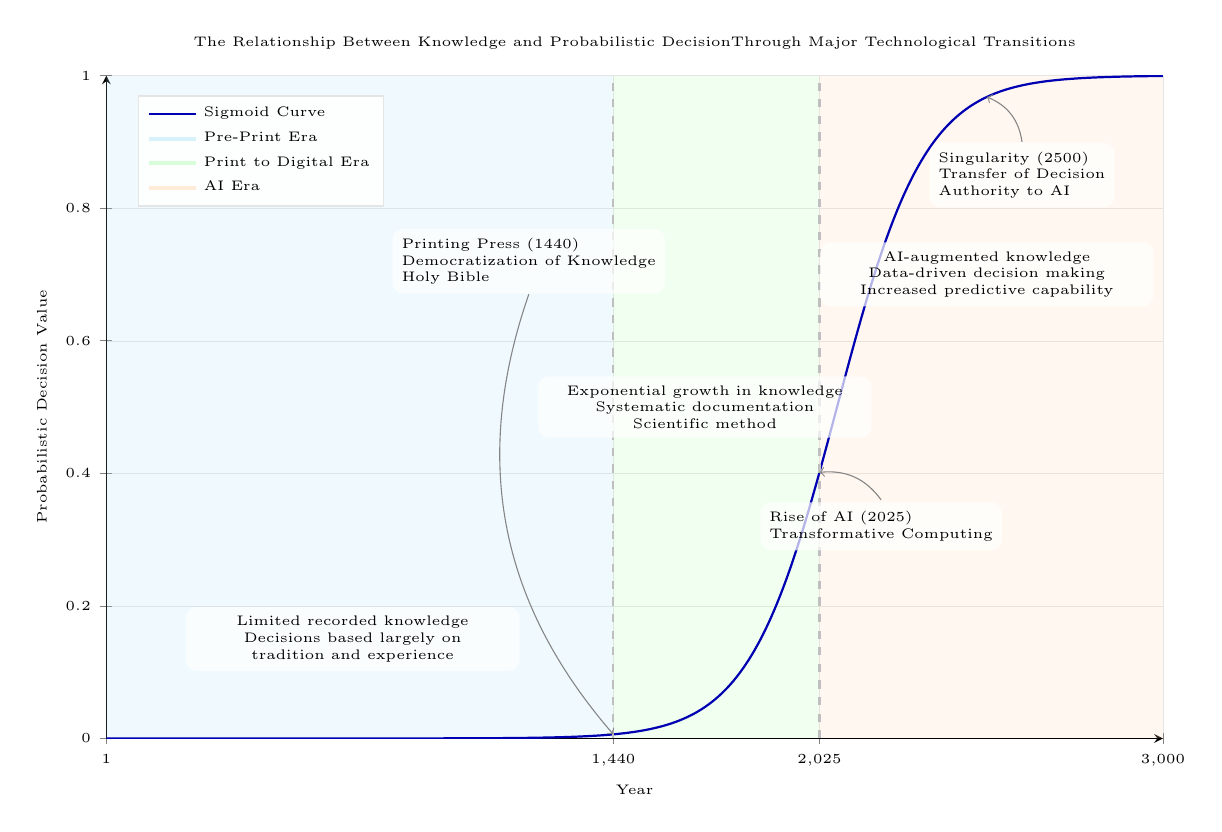
\begin{tikzpicture}
		\begin{axis}[
			width=15cm,
			height=10cm,
			xlabel={\tiny Year},
			ylabel={\tiny Probabilistic Decision Value},
			title={\tiny The Relationship Between Knowledge and Probabilistic Decision\\\tiny Through Major Technological Transitions},
			legend pos=north west,
			legend cell align={left},
			ymin=0, ymax=1,
			xmin=1, xmax=3000,
			xtick={1, 1440, 2025, 3000},
			ytick={0, 0.2, 0.4, 0.6, 0.8, 1.0},
			grid=major,
			grid style={line width=.1pt, draw=gray!20},
			axis lines=left,
			tick label style={font=\tiny},
			legend style={
				fill=white,
				fill opacity=0.9,
				draw=gray!20,
				text opacity=1,
				font=\tiny
			},
			every axis plot/.append style={line width=1.5pt}
			]
			% Background regions first (before the main plot)
			% Pre-Print Era
			\fill[cyan!30, opacity=0.2] (axis cs:1,0) rectangle (axis cs:1440,1);
			
			% Print to Digital Era
			\fill[green!30, opacity=0.2] (axis cs:1440,0) rectangle (axis cs:2025,1);
			
			% AI Era
			\fill[orange!30, opacity=0.2] (axis cs:2025,0) rectangle (axis cs:3000,1);
			
			% Main sigmoid curve
			\addplot [domain=1:3000, samples=200, smooth, thick, blue!70!black] {1 / (1 + exp(-(x - 2075) / 125))};
			\addlegendentry{Sigmoid Curve}
			
			% Add legend entries for regions
			\addplot[cyan!30, opacity=0.5] coordinates {(0,0) (0,0)}; % Dummy plot for legend
			\addlegendentry{Pre-Print Era}
			
			\addplot[green!30, opacity=0.5] coordinates {(0,0) (0,0)}; % Dummy plot for legend
			\addlegendentry{Print to Digital Era}
			
			\addplot[orange!30, opacity=0.5] coordinates {(0,0) (0,0)}; % Dummy plot for legend
			\addlegendentry{AI Era}
			
			% Transition lines with improved styling
			\draw[dashed, thick, gray!50] (axis cs:1440,0) -- (axis cs:1440,1);
			\draw[dashed, thick, gray!50] (axis cs:2025,0) -- (axis cs:2025,1);
			
			% Enhanced annotations with background
			\node[align=center, font=\tiny, fill=white, fill opacity=0.7, text opacity=1, rounded corners, 
			text width=4cm] at (axis cs:700, 0.15) 
			{Limited recorded knowledge\\Decisions based largely on tradition and experience};
			
			\node[align=center, font=\tiny, fill=white, fill opacity=0.7, text opacity=1, rounded corners,
			text width=4cm] at (axis cs:1700, 0.5) 
			{Exponential growth in knowledge\\Systematic documentation\\Scientific method};
			
			\node[align=center, font=\tiny, fill=white, fill opacity=0.7, text opacity=1, rounded corners,
			text width=4cm] at (axis cs:2500, 0.7) 
			{AI-augmented knowledge\\Data-driven decision making\\Increased predictive capability};
			
			% Key events with curved arrows
			\draw[line width=0.4pt, <-, lightgray!70!black, out=135, in=-45] 
			(axis cs:1440, {1 / (1 + exp(-(1440 - 2075) / 125))}) 
			to[bend left] (axis cs:1200, 0.67);
			\node[align=left, font=\tiny, fill=white, fill opacity=0.7, text opacity=1, rounded corners]
			at (axis cs:1200, 0.72) 
			{Printing Press (1440)\\Democratization of Knowledge\\Holy Bible};
			
			\draw[line width=0.4pt, <-, lightgray!70!black, out=135, in=-45] 
			(axis cs:2025, {1 / (1 + exp(-(2025 - 2075) / 125))}) 
			to[bend left] (axis cs:2200, 0.36);
			\node[align=left, font=\tiny, fill=white, fill opacity=0.7, text opacity=1, rounded corners]
			at (axis cs:2200, 0.32) 
			{Rise of AI (2025)\\Transformative Computing};
			
			\draw[line width=0.4pt, <-, lightgray!70!black, out=135, in=-45] 
			(axis cs:2500, {1 / (1 + exp(-(2500 - 2075) / 125))}) 
			to[bend left] (axis cs:2600, 0.9);
			\node[align=left, font=\tiny, fill=white, fill opacity=0.7, text opacity=1, rounded corners]
			at (axis cs:2600, 0.85) 
			{Singularity (2500)\\Transfer of Decision\\Authority to AI};			
			
		\end{axis}
	\end{tikzpicture}
\end{document}